\documentclass[12pt, fullpage,letterpaper]{article}

% I copied older latex files that include packages we may need but idk,
% I'm not too knowledgeable about all things Latex
\usepackage[margin=1in]{geometry}
\usepackage{url}
\usepackage{amsmath}
\usepackage{amssymb}
\usepackage{amsthm}
\usepackage{xspace}
\usepackage{graphicx}
\usepackage{hyperref}
\usepackage{listings}
\usepackage{bm}
\usepackage{cite}
\usepackage{subfigure}
\usepackage{cite}

\theoremstyle{definition}
\newtheorem{definition}{Definition}[section]

\graphicspath{{./}}
\title{Final Report}
\author{Tyler Adams: u0761872 \\Corbin Baldwin: u0292800}

\begin{document}
	\maketitle 
	\hrule 
	\vskip 0.5cm
	\section{Paper Rubric}
	\begin{enumerate}
		\item Team Members:  the names and UID of your team members.
		\item Introduction:  Motivation  and  a  brief  project  description.   What  is  the  main  objective  of  your project?  What is an overview of your strategy to achieve your objective?
		\item Technical Contributions:  What are the technical contributions of your proposed work?
		\item Data:  What are the type(s) of data your project will be dealing with?  How do you plan to gethold of such data sets?  What kind of insights are you planning to obtain from your data?
		\item Background and Related Work:  technical background, together with related work.  What are thestate-of-the-art techniques in dealing with the data of your interest?  What are the differences andsimilarities between your work and the state-of-the-art?
		\item Methods:   What  methods  have  you  used/developed?   What  are  your  strategies  in  tackling  the proposed problem?
		\item Results and Insights:  What are the results of your proposed project?  What are the key insights?
		\item Evaluation:  What metrics do you use to evaluate how successful your project is?  What are thetake home messages based on your evaluation?
		\item Deliverables:  What are your deliverables?  (e.g.  source code,  video demo,  etc.)  What software(and possibly hardware) do you use?  Or in the case you are working on software extensions, whatis the baseline software you work with?
		\item Conclusions and Dicussions:  answer specific questions below using 1-2 sentences:
		\begin{itemize}
			\item What is an overview of your project?
			\item What are your project objectives?
			\item What questions does your project address?
			\item What are the key insights based on your results?
			\item What are future directions?
		\end{itemize}
	\end{enumerate}	
	
	\section*{\normalfont Introduction}
	% Motivation and a brief project description.
	Rayleigh-Taylor instability (RTI) forms at the surface of contact between two fluids, one of which is denser and accelerates toward the other. Formations in RTI are not symmetric between the denser and lighter fluids, and the features of both sides serve to characterize the RTI. However, these features quickly rise in complexity, and it is unrealistic to simulate them beyond a given time threshold. In our project we hope to use machine-learning to construct a classifier that accurately predicts the mixing-specie using topological data analysis (TDA) and other methods learned throughout the course. To do so, we will compare two different data structures on which we will train various classifiers. The first uses persistence diagrams constructed using persistent homology on the mixing boundary. The second is constructed on the mixing boundary using what we later define as \emph{critical diagrams}. This path is inspired directly by the material we have learned throughout the course. We will compare the various classifiers and their results using resources and software developed for the second course project.
	
	\section*{\normalfont Technical Contributions} 
	\section*{\normalfont Data}
	The data we used was simulated using the Palabos library, located at \url{http://www.palabos.org/}. This library specializes in modeling fluid dynamics. A \emph{mixing class} is an ordered pair $(\rho_1, \rho_0)$ of densities of fluids whereby $\rho_1$ is the density of the heavier top fluid and $\rho_0$ is the density of the lighter bottom fluid. Using the above mentioned software, we chose four mixing classes, 
	$$
		(1.0, 0.0), \ \ (0.8, 0.0), \ \ (1.0, 0.2), \ \ (0.8, 0.2)
	$$
	and for each mixing class we ran 10 simulations. Each simulation had a different randomly generated initial condition leading to different mixing behavior. Both mixing classes $(1.0, 0.0), (0.8, 0.0)$ had 51 images generated during the simulation. The mixing class $(1.0, 0.2)$ had 71 images per simulation and the mixing class $(0.8, 0.2)$ had 67 images per simulation. These images, in \texttt{.gif} format, were the source of our data for the entire project. 
	
	We were unable to use more mixing classes because of the amount of time it takes to run the software and extract boundaries as well as the fact that we were unable to develop robust boundary extraction software for some of the more wild images generated for other mixing specie. Additionally, the densities above are purely numeric. No fluid has a density of 0.0. However the software mentioned above would break whenever we used density values outside the interval $[0.0, 1.0]$ so we were restricted to this range. Thus the fluid densities do not represent actually existing fluids. 
	
	\section*{\normalfont Background and Related Work}
	The inspiration for the project largely came from \cite{paper}. In the paper, the authors simulate RTI and keep track of the bubble evolution using Morse-Smale Complexes. Since we are using two-dimensional images, we do not believe Morse-Smale complexes are well-defined so we did not directly use their approach. In tracking bubble evolution to display a merge-split tree, the authors kept track of the critical point locations (maximum critical points, not minimum critical points) by using the Euclidean distance between critical points in successive time steps of the simulation. Given some threshold (Euclidean radius), it seemed that they treated two critical points in two successive simulations if they were within this threshold. This was the inspiration for our method of attack as described in the section below. 
	
	We are not aware of any work that tries to classify mixing specie using a machine learning approach. Because of this, we are unable to compare our approach with a state-of-the-art baseline. In lieu of this, because our approach is almost algorithmically-identical to the use of peristent homology in classifying images with which this course gave us much experience, we chose that as our baseline of comparison.  
	
	\section*{\normalfont Methods}
	\subsection*{\normalfont Boundary Extraction} Given images, we
	\subsection*{\normalfont Persistent Homology}
	For the baseline, we chose the latest images in each simulation for each class as the choice object with which to calculate persistent homology. For example, if we let a simulation run 6000 iterations, we chose the image generated at time 6000 as a representative of this simulation. With this image, we extracted the boundary and computed 0 and 1-dimensional persistent homology and their corresponding persistence diagrams using Ripser. Using these persistence diagrams, we trained classifiers learned throughout the course. The results are discussed in the Results and Insights section below.
	
	\subsection*{\normalfont Critical Diagrams} 
	While persistence diagrams are multi-sets with a certain structure not necessarily dependent on homology, we wish to define critical diagrams in the same way but to differentiate their connotation with persistent homology. In \cite{Hofer}, a persistence diagram is defined as follows:
	\theoremstyle{definition}
	\begin{definition}
		Let $\Delta = \{ x\in \mathbb{R}^2_{\Delta} : \textrm{mult}(x) = \infty \}$ be the multiset of the diagonal $\mathbb{R}^2_{\Delta} = \{ (x_0, x_1) \in \mathbb{R}^2 : x_1 = x_0 \}$, where $\textrm{mult}$ deontes the multiplicity function and let $\mathbb{R}_{\star}^2 = \{ (x_0, x_1) \in \mathbb{R}^2 : x_1 > x_0 \}$. A \emph{persistence diagram}, $\mathcal{D}$, is a multiset of the form
		$$
			\mathcal{D} = \{x: x \in \mathbb{R}_{\star}^2  \} \cup \Delta.
		$$
	\end{definition}
	Unfortunately in our presentation we did not make this point clear. We define a \emph{critical diagram} to be exactly identical to a persistence diagram as in Definition 1.1 but we strip it of any connotation to persistent homology. With this clarification, because they have the same mathematical structure we may use software developed for persistence diagrams on critical diagrams. 
	
	Continuing, given any two successive time-steps in a simulation of RTI, say $t$ and $t + 1$, we first extract the boundaries of the two images generated by the simulation at times $t$ and $t + 1$. Assuming a parameterization of the boundary points, we then find the critical points of the boundary for both images. That is, we find the finite differences between every two successive boundary points taking into account division by zero. We then determine whether the type of the critical point is a local minimum or local maximum and we store its type and its position. Saddle points are ignored and not considered critical points. 
	
	Given a threshold, say a squared pixel radius of $\epsilon^2$, a critical point $c_{t + 1} = (x_{t + 1}, y_{t + 1} )$ at time $t + 1$ is considered \emph{equal} to a critical point $c_t = (x_t, y_t)$ at time $t$ if they share the same critical point type and $d_E(c_t, c_{t + 1})^2 < \epsilon^2$ where $d_E$ is the Euclidean metric. If two critical points are considered equal, we set both their birth times to the earlier of the respective birth times. If a critical point $c_{t + 1}$ is not equal to any point in the set of critical points at $t$, then $c_{t + 1}$ is considered \emph{born} and its birth time is $t + 1$. If a critical point $c_t$ is not equal to any point in the set of critical points at $t + 1$, then we consider $c_t$ to have \emph{died}. In both birth and deaths we store the iteration where the birth or death occured. 
	
	Note that if many critical points are within the threshold or if they form a chain, they will all be considered the same critical point. This is where the euclidean distance hyper-parameter is important. If a critical point has not died by the end of the simulation we set its death time to the total number of steps in the simulation. Importantly, every critical point has a death time that takes place \emph{after} its birth time. The set of distinct birth/death pairs for each critical point (up to equivalence) can then be formed into a critical diagram. Our hope was that this construction can somewhat accurately capture the evolution of the mixing fluid which is a very important feature of mixing specie, a feature that we do not personally know how to capture with persistent homology. We then use the critical diagrams to develop the same type of classifiers used for persistent homology. The results are discussed in the section below.
	
	\section*{\normalfont Results and Insights}
	\section*{\normalfont Evaluation}
	\section*{\normalfont Deliverables} 
	\section*{\normalfont Conclusions and Discussions}
	
%		\begin{figure*}[ht!]
%		\centering
%		\begin{subfigure}
%			\centering
%			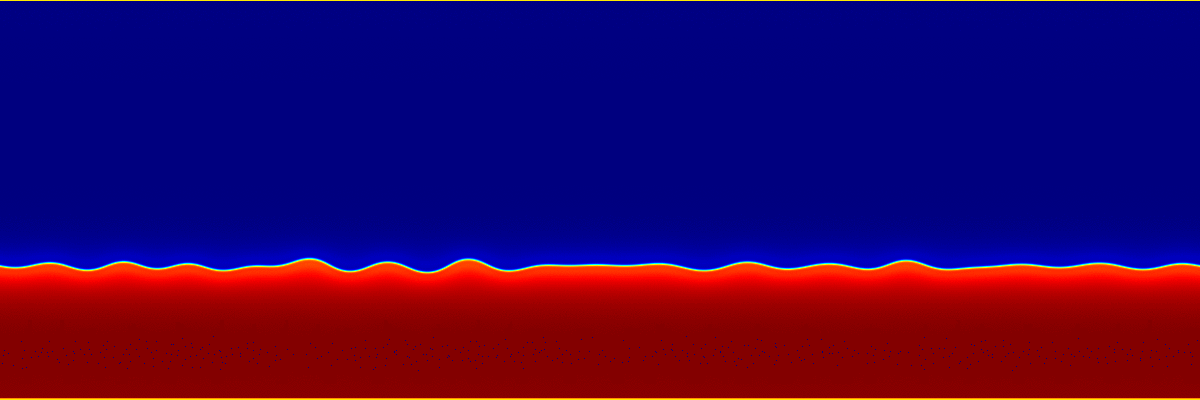
\includegraphics[scale = .25]{fig1.png}
%			\caption{$t = 2100$}
%		\end{subfigure}
%		\begin{subfigure}
%			\centering
%			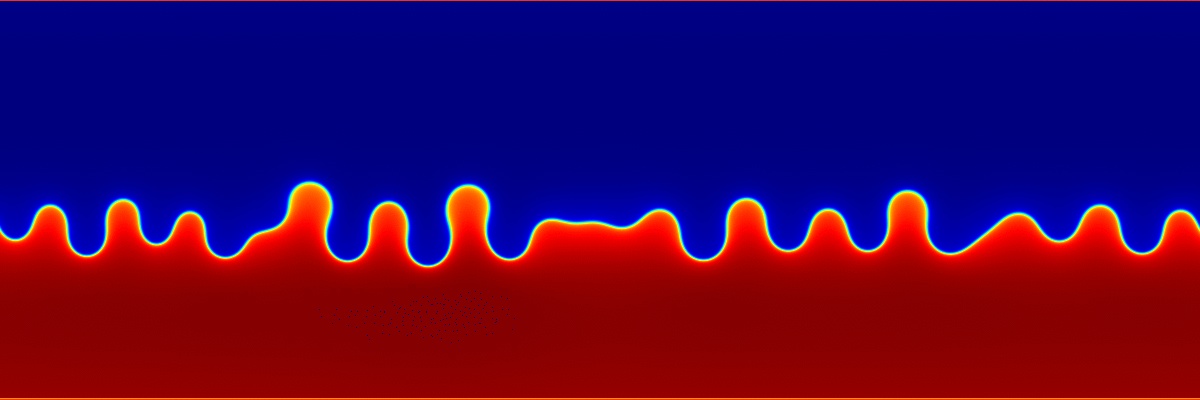
\includegraphics[scale = .25]{fig2.png}
%			\caption{$t = 2600$}
%		\end{subfigure}
%		\begin{subfigure}
%			\centering
%			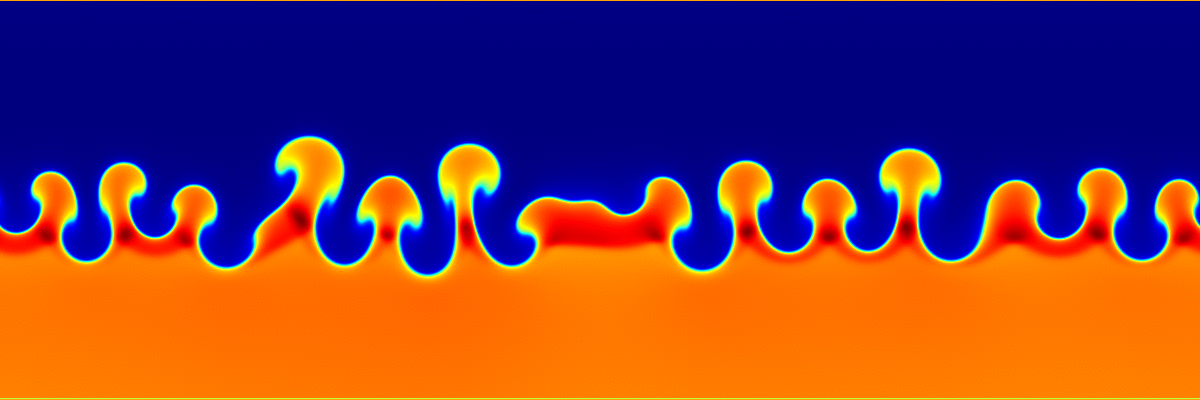
\includegraphics[scale = .25]{fig3.png}
%			\caption{$t = 2900$}
%		\end{subfigure}
%		\begin{subfigure}
%			\centering
%			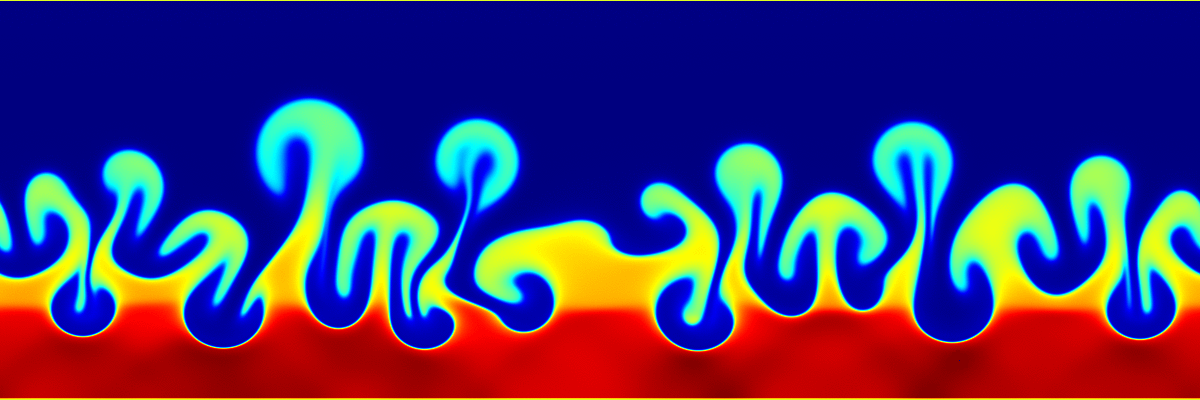
\includegraphics[scale = .25]{fig4.png}
%			\caption{$t = 3300$}
%		\end{subfigure}
%	\end{figure*}
%	
	
%	\section*{\normalfont Upcoming Milestones} The next milestones are:
%	\begin{enumerate}
%%		\item Smooth out the isosurfaces so that we can better track bubble evolution.
%		\item Implement a height function to track critical points and the evolution of bubbles.
%		\item Construct a persistence diagram describing the birth and death of bubbles.
%		\item Possibly classify simulations by density or other parameters by their persistence diagrams. I.e., is this bubble evolution symptomatic of the mixing of air and water?
%	\end{enumerate} 
%
%	\section*{\normalfont Preliminary Results}
%	While we have not applied a proper topological filtration, we have extracted some data that will be necessary in the final stages. The most challenging aspect so far has been finding a valid, practical algorithm for running the simulation of an RTI. As shown above, we have managed to get one working that provides a solution to the problem in the two dimensional case. With the images that are output, we can approximate the isosurface using edge-detecting algorithms, which we have also done.
%	
%	\section*{\normalfont Modifications} RTI is a difficult to simulate on a large scale as it involves numerically solving the system of PDE's
%	
%	\begin{gather*}
%		\frac{\partial \rho Y_i}{\partial t} + \nabla \cdot (\rho Y_i \vec{u} + \vec{J}_i) = 0; i = 1, 2 \\
%		\frac{\partial \rho \vec{u}}{\partial t} + \nabla \cdot (\rho \vec{u} \cdot \vec{u} + p \vec{\vec{\delta}} - \vec{\vec{\tau}}) = \rho \vec{g} \\
%		\frac{\partial E}{\partial t} + \nabla \cdot ((E + p)\vec{u} -\vec{\vec{\tau}}\cdot \vec{u} + \vec{q_c} + \vec{q_d} ) = \rho \vec{g} \cdot \vec{u} \\
%	\end{gather*} 
%	at each time step. While we have some background in PDE's, we do not feel our background is sufficient to construct a solver from scratch quickly. After researching a few algorithms and trying to implement broken software, we found the Palabos library, located at \url{http://www.palabos.org/}, which contains the software used to generate the images above. Due to the computation intensive process of generating a 3D dataset on which to use Morse-Smale complexes, we may choose to use the 2-dimensional version. If we use 2D, we will use a height function to compute and store relevant critical point information. Additionally, since we are in essence extracting a boundary from the 2D sample image, we can use methods learned in this class to attempt to classify different mixing species using TDA and machine-learning. Alternatively, if we can generate sufficient 3D data, we can use the recommended software to continue with the project as originally planned.
%	
%	 	\section*{\normalfont Summary}
%	We have arranged a process to acquire the data necessary for our research over two dimensional RTIs, including the simulation and the extraction of isosurfaces from said simulation. We hope to acquire three dimensional RTI data as well. Regarding the data, we still have not utilized topological data analysis to perform the essence of our research. This should include several topological filtrations.
%	
%	With the filtrations we plan to classify simulations by the structure of their RTIs. Factors that will be considered include the birth and death times of bubbles, as well as their size.
\bibliography{mybib}{}
\bibliographystyle{plain}

\end{document}
